\chapter{Appendices}
\label{chap:appendix}
\appendix

\paragraph{Outline}

This appendix gathers all the supplementary material of \Cref{chapter:nips} and goes as follows: \Cref{sec:proofs} details all the proofs of the main results. \Cref{sec:params:appendix} lists the parameters used in the experiments. \Cref{subsubsec:instruction-reproducibility} provides instruction to reproduce the experiments. Finally we fill the \acrlong{ML} Reproducibility Checklist and we justify each statement in \Cref{sec:ml-checklist}.


\section{Proofs of Main Results}
\label{sec:proofs}

\subsection{\Cref{prop:bellman-expectation}}
\label{proof-bellman-expectation}

\begin{proof}
    This proof is the same as that in classical multi-objective MDPs.

    \begin{align*}
        \oV^{\budgetedpolicy}(\os) &\eqdef \expectedvalue\left[ \augmentedreturn^{\budgetedpolicy} \condbar \ov{s_0} = \os\right] \\
        &=\sum_{\oa\in\ocA} \probability{\oa_0 = \oa \condbar\ov{s_0} = \os} \expectedvalue\left[ \augmentedreturn^{\budgetedpolicy} \condbar \ov{s_0} = \os, \oa_0 = \oa\right]\\
        &= \sum_{\oa\in\ocA} \budgetedpolicy(\oa | \os) \oQ^{\budgetedpolicy}(\os,\oa).
    \end{align*}
    \begin{align*}
        \oQ^{\budgetedpolicy}(\os, \oa) &\eqdef \expectedvalue\left[\sum_{t=0}^\infty \discountfactor^t \augmentedreward(\os_t, \oa_t)\condbar \ov{s_0} = \os, \ov{a_0} = \oa\right] \\
        &= \augmentedreward(\os, \oa) + \sum_{\os'\in\ocS}\probability{\os_1 = \os' \condbar\ov{s_0} = \os, \ov{a_0} = \oa}\cdot \expectedvalue\left[\sum_{t=1}^\infty \discountfactor^t \augmentedreward(\os_t, \oa_t)\condbar \ov{s_1} = \os'\right] \\
        &= \augmentedreward(\os, \oa) + \discountfactor\sum_{\os'\in\ocS}\augmentedtransition\left(\os' \condbar\os, \oa\right) \expectedvalue\left[\sum_{t=0}^\infty \discountfactor^t \augmentedreward(\os_t, \oa_t) \condbar \ov{s_0} = \os'\right] \\
        &= \augmentedreward(\os, \oa) + \discountfactor\sum_{\os'\in\ocS}\augmentedtransition\left(\os' \condbar\os, \oa\right) \oV^{\budgetedpolicy}(\os').
    \end{align*}

    \textbf{Contraction of $\abo^{\budgetedpolicy}$:}
    Let $\budgetedpolicy\in\policies, \oQ_1, \oQ_2\in(\Real^2)^{\ocS\ocA}$.
    \begin{align*}
        \forall \os\in\ocS, \oa\in\ocA,\quad \left|\abo^{\budgetedpolicy} \oQ_1(\os,\oa) - \abo^{\budgetedpolicy} \oQ_2(\os,\oa)\right| &= \left|\discountfactor\expectedvalueover{\substack{\os'\sim\augmentedtransition(\os'|\os,\oa) \\ \oa'\sim\budgetedpolicy(\oa'|\os')}} \oQ_1(\os',\oa') - \oQ_2(\os',\oa')\right|\\
        &\leq \discountfactor\left\|\oQ_1-\oQ_2\right\|_\infty.
    \end{align*}
    Hence, $\left\|\abo^{\budgetedpolicy} \oQ_1 - \abo^{\budgetedpolicy} \oQ_2 \right\|_\infty \leq \discountfactor\left\|\oQ_1-\oQ_2\right\|_\infty$

    According to the Banach fixed point theorem, $\abo^{\budgetedpolicy}$ admits a unique fixed point.
    It can be easily verified that $\oQ^{\budgetedpolicy}$ is indeed this fixed point by combining the two Bellman Expectation equations~\eqref{eq:bellman_expectation}.
\end{proof}

\subsection{\Cref{thm:bellman-optimality}}
\label{proof-thm:bellman-optimality}

\begin{proof}
    Let $\os, \oa \in \ocA\times\ocS$. For this proof, we consider potentially non-stationary policies $\budgetedpolicy=(\rho, \budgetedpolicy')$, with $\rho\in\cM(\ocA)$, $\budgetedpolicy'\in\cM(\ocA)^\Natural$. The results will apply to the particular case of stationary optimal policies, when they exist.

    \begin{align}
        \Qr^*(\os, \oa) &=  \max_{\rho, \budgetedpolicy'} \Qr^{\rho, \budgetedpolicy'}(\os', \oa') \label{eq:pthm_def}\\
        &= \max_{\rho, \budgetedpolicy'} \reward(s, a) + \discountfactor \sum_{\os'\in\ocS} \augmentedtransition(\os' | \os, \oa) \Vr^{\rho, \budgetedpolicy'}(\os') \label{eq:pthm_exp}\\
        &= \reward(s, a) + \discountfactor \sum_{\os'\in\ocS}  \augmentedtransition(\os' | \os, \oa) \max_{\rho, \budgetedpolicy'} \sum_{\oa'\in\ocA} \rho(\oa' | \os')\Qr^{\budgetedpolicy'}(\os', \oa') \label{eq:pthm_marg}\\
        &= \reward(s, a) + \discountfactor \sum_{\os'\in\ocS}  \augmentedtransition(\os' | \os, \oa) \max_\rho\sum_{\oa'\in\ocA}\rho(\oa' | \os')\max_{\budgetedpolicy'\in\policies_a(\os')}\Qr^{\budgetedpolicy'}(\os', \oa') \label{eq:pthm_max}\\
        &= \reward(s, a) + \discountfactor \sum_{\os'\in\ocS}  \augmentedtransition(\os' | \os, \oa) \max_\rho\expectedvalueover{\oa'\sim\rho}\Qr^*(\os', \oa') \label{eq:pthm_marg_def2}
    \end{align}
    where $\budgetedpolicy = (\rho, \budgetedpolicy')\in\policies_a(\os)$ and $\budgetedpolicy'\in\policies_a(\os')$.

    This follows from:
    \begin{enumerate}
        \item[\eqref{eq:pthm_def}.] Definition of $\oQ^*$.
        \item[\eqref{eq:pthm_exp}.] Bellman Expectation expansion from \Cref{prop:bellman-expectation}.
        \item[\eqref{eq:pthm_marg}.] Marginalisation on $\oa'$.
        \item[\eqref{eq:pthm_max}.] \begin{itemize}
                                        \item Trivially $\max_{\budgetedpolicy'\in\policies_a(\os')} \sum_{\oa'\in\ocA} \cdot \leq \sum_{\oa'\in\ocA} \max_{ \budgetedpolicy'\in\policies_a(\os)} \cdot$.
                                        \item Let $\ov{\budgetedpolicy}\in\argmax_{\budgetedpolicy'\in\policies_a(\os')} \Qr^{\budgetedpolicy'}(\os', \oa')$, then:
                                        \begin{align*}
                                            \sum_{\oa'\in\ocA}\rho(\oa'|\os')\max_{\budgetedpolicy'\in\policies_a(\os')}\Qr^{\budgetedpolicy'}(\os', \oa') &= \sum_{\oa'\in\ocA}\rho(\oa'|\os')\Qr^{\ov{\budgetedpolicy}}(\os', \oa') \\
                                            &\leq  \max_{\budgetedpolicy'\in\policies_a(\os')} \sum_{\oa'\in\ocA}\rho(\oa'|\os')\Qr^{\budgetedpolicy'}(\os', \oa').
                                        \end{align*}
        \end{itemize}
        \item[\eqref{eq:pthm_marg_def2}.] Definition of $\oQ^*$.
    \end{enumerate}

    Moreover, the condition $\budgetedpolicy=(\rho, \budgetedpolicy')\in\policies_a(\os)$ gives
    \begin{equation*}
        \expectedvalueover{\oa'\sim\rho} \Qc^{*}(\os, \oa) = \expectedvalueover{\oa'\sim\rho} \Qc^{\budgetedpolicy'}(\os, \oa) = \Vc^{\budgetedpolicy}(\os) \leq \budget.
    \end{equation*}

    Consequently, $\budgetedpolicy_\text{greedy}(\cdot; \oQ^*)$ belongs to the $\argmax$ of \eqref{eq:pthm_marg_def2}, and in particular:
    \begin{equation*}
        \Qr^*(\os, \oa) = r(\os, \oa) + \discountfactor \sum_{\os'\in\ocS}  P(\os' | \os, \oa) \expectedvalueover{\oa'\sim\budgetedpolicy_\text{greedy}(\os', \oQ^*)} \Qr^*(\os', \oa').
    \end{equation*}

    The same reasoning can be made for $\Qc^*$ by replacing $\max$ operators by $\min$, and $\policies_a$ by $\policies_r$.

\end{proof}


\subsection{\Cref{prop:greedy_optimal}}
\label{proof-prop:greedy_optimal}

\begin{proof}
    Notice from the definitions of $\abo^{*}$ and $\abo^{\budgetedpolicy}$ in \eqref{eq:bellman-optimality} and \eqref{eq:bellman_expectation_operator} that $\abo^{*}$ and $\abo^{\budgetedpolicy_\text{greedy}(\cdot;\oQ^*)}$ coincide on $\oQ^*$. Moreover, since $\oQ^* = \abo^{*}\oQ^*$ by \Cref{thm:bellman-optimality}, we have: $\abo^{\budgetedpolicy_\text{greedy}(\cdot;\oQ^*)} \oQ^* = \abo^{*} \oQ^* = \oQ^*
    $.
    Hence, $\oQ^*$ is a fixed point of $\abo^{\budgetedpolicy_\text{greedy}(\cdot;\oQ^*)}$, and by \Cref{prop:bellman-expectation} it must be equal to $\oQ^{\budgetedpolicy_\text{greedy}(\cdot;\oQ^*)}$

    To show the same result for $\oV^*$, notice that
    \begin{equation*}
        \oV^{\budgetedpolicy_\text{greedy}(\oQ^*)}(\os) = \expectedvalueover{\oa\sim\budgetedpolicy_\text{greedy}(\oQ^*)}\oQ^{\budgetedpolicy_\text{greedy}(\oQ^*)}(\os,\oa) = \expectedvalueover{\oa\sim\budgetedpolicy_\text{greedy}(\oQ^*)}\oQ^*(\os,\oa).
    \end{equation*}
    By applying the definitions of $\oQ^*$ and $\budgetedpolicy_\text{greedy}$, we recover the definition of $\oV^*$.
\end{proof}

\subsection{\Cref{thm:contraction}}
\label{proof-thm:contraction}

\begin{proof}
    In the trivial case $|\cA| = 1$, there exits only one policy $\budgetedpolicy$ and $\abo^{*}= \abo^{\budgetedpolicy}$, which is a contraction by \Cref{prop:bellman-expectation}.

    In the general case $|\cA| \geq 2$, we can build the following counter-example:

    Let $(\cS, \cA, \transition, \reward, \constraint)$ be a \gls{BMDP}.
    For any $0 < \extrasmallvalue < 1$, we define $\oQ_{\extrasmallvalue}^1$ and $\oQ_{\extrasmallvalue}^2$ as:

    \begin{align*}
        \oQ_{\extrasmallvalue}^1(\os,\oa) =
        \begin{cases}
            (0, 1), & \text{if } a = a_0 \\
            (\frac{1}{{\extrasmallvalue}}, 1+{\extrasmallvalue}), & \text{if } a \neq a_0
        \end{cases}\\
        \oQ_{\extrasmallvalue}^2(\os,\oa) =
        \begin{cases}
            (1, 0), & \text{if } a = a_0 \\
            (1+\frac{1}{{\extrasmallvalue}}, {\extrasmallvalue}), & \text{if } a \neq a_0
        \end{cases}
    \end{align*}
    Then, $\|\oQ_1-\oQ_2\|_\infty = 1$.
    $\oQ_{\extrasmallvalue}^1$ and $\oQ_{\extrasmallvalue}^2$ are represented in \Cref{fig:concavity_example}.

    \begin{figure}[tp]
        \centering
        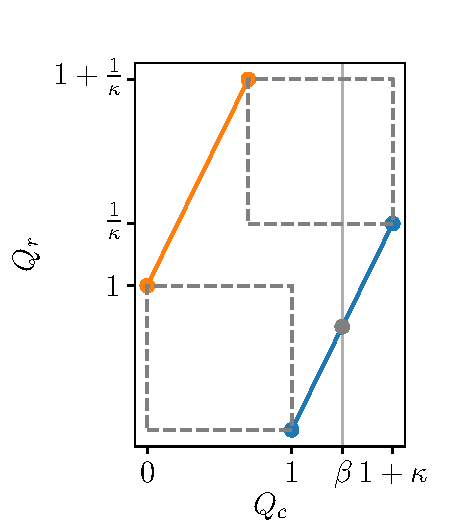
\includegraphics[width=0.5\textwidth]{sources/appendix/source/img/concavity_example.pdf}
        \caption[Concavity Example]{Representation of $\oQ_{\extrasmallvalue}^1$ (blue) and $\oQ_{\extrasmallvalue}^2$ (orange)}
        \label{fig:concavity_example}
    \end{figure}

    But for $\oa=(a,\budgetaction)$ with $\budgetaction = 1+{\extrasmallvalue}/2$, we have:
    \begin{align*}
        \|\abo^{*}\oQ_{\extrasmallvalue}^1(\os, \oa) - &\abo^{*}\oQ_{\extrasmallvalue}^2(\os, \oa)\|_\infty \\
        &=\discountfactor\left\|\expectedvalueover{\os'\sim\augmentedtransition(\os'|\os,\oa)} \expectedvalueover{\oa'\sim\budgetedpolicy_\text{greedy}(\oQ^1_{\extrasmallvalue})}\oQ^1_{\extrasmallvalue}(\os',\oa') - \expectedvalueover{\oa'\sim\budgetedpolicy_\text{greedy}(\oQ^2_{\extrasmallvalue})}\oQ^2_{\extrasmallvalue}(\os',\oa')\right\|_\infty \\
        &= \discountfactor\left\|\expectedvalueover{\os'\sim\augmentedtransition(\os'|\os,\oa)}(\frac{1}{2{\extrasmallvalue}}, 1+\frac{{\extrasmallvalue}}{2}) - (1+\frac{1}{{\extrasmallvalue}},{\extrasmallvalue} )\right\|_\infty \\
        &= \discountfactor(1+\frac{1}{2{\extrasmallvalue}}).
    \end{align*}

    Hence, $\|\abo^{*}\oQ_{\extrasmallvalue}^1 - \abo^{*}\oQ_{\extrasmallvalue}^2\|_\infty \geq \discountfactor(1+\frac{1}{2{\extrasmallvalue}})$.

    As a conclusion, there does not exist $L>0$ such that:
    $$\forall \oQ_1,\oQ_2\in(\Real^2)^{\ocS\ocA}, \|\abo^{*}\oQ^1 - \abo^{*}\oQ^2\|_\infty \leq L \|\oQ^1 - \oQ^2\|_\infty$$
    In other words, $\abo^{*}$ is not a contraction for $\|\cdot\|_\infty$.
\end{proof}

\subsection{\Cref{thm:contractivity-smooth}}
\label{proof-contraction-with-smooth}

\begin{remark}
    This proof makes use of insights detailed in the proof of \Cref{prop:bftq_pi_hull} (\Cref{sec:proof_pi_hull}), which we recommend the reader to consult first.
\end{remark}

\begin{proof}
    We now study the contractivity of $\abo^{*}$ when restricted to the functions of $\cL_{\discountfactor}$ defined as follows:

    \begin{equation}
        \cL_{\discountfactor} = \left\{\begin{array}{cc}

                                           \oQ\in(\Real^2)^{\ocS\ocA}\text{ s.t. }\exists L<\frac{1}{\discountfactor}-1: \forall \os\in\ocS,\oa_1,\oa_2\in\ocA,   \\

                                           |\Qr(\os,\oa_1) - \Qr(\os,\oa_2)| \leq L|\Qc(\os,\oa_1) - \Qc(\os,\oa_2)|
        \end{array}\right\}.
    \end{equation}
    That is, for all state $\os$, the set $\oQ(\os, \ocA)$ plot in the $(\Qc,\Qr)$ plane must be the \emph{graph} of a $L$-Lipschitz function, with $L<1/\discountfactor-1$.

    We impose such structure for the following reason: the counter-example presented above prevented contraction because it was a pathological case in which the slope of $\oQ$ can be arbitrary large. As a consequence, when solving $\Qr^*$ such that $\Qc^*=\budget$, a vertical slice of a $\|\cdot\|_\infty$ ball around $\oQ_1$ (which must contain $\oQ_2$) can be arbitrary large as well.


    We denote $\text{Ball}(\oQ,R)$ the ball of centre $\oQ$ and radius $R$ for the $\|\cdot\|_\infty$-norm:
    \begin{equation*}
        \text{Ball}(\oQ,R) = \{\oQ'\in(R^2)^{\ocS\ocA}: \|\oQ-\oQ'\|_\infty \leq R\}.
    \end{equation*}

    We give the three main steps required to show that $\abo^{*}$ restricted to $\cL_{\discountfactor}$ is a contraction. Given $\oQ^1, \oQ^2\in\cL_{\discountfactor}$, show that:

    \begin{enumerate}
        \item $\oQ^2\in\text{Ball}(\oQ^1,R)\implies\cF^2\in\text{Ball}(\cF^1, R), \forall\os\in\ocS$, where $\cF$ is the top frontier of the convex hull of undominated points, as defined in~\Cref{sec:proof_pi_hull}.
        \item $\oQ\in\cL_{\discountfactor} \implies \cF$ is the graph of a $L$-Lipschitz function, $\forall\os\in\ocS$.
        \item taking the slice $\Qc=\budget$ of a ball $\text{Ball}(\cF,R)$ with $\cF$ $L$-Lipschitz results in an interval on $\Qr$ of range at most $(L+1)R$
    \end{enumerate}

    These three steps will allow us to control $\Qr^{2*} - \Qr^{1*}$ as a function of $R = \|\oQ^2-\oQ^1\|_\infty$.

    \paragraph{Step 1}

    We want to show that if $\oQ^1$ and $\oQ^2$ are close, then $\cF^1$ are $\cF^2$ are close as well in the following sense:

    \begin{align}
        \cF^2\in\text{Ball}(\cF^1, R) &\iff d(\cF^1, \cF^2) \leq R \iff \max_{q^2\in\cF^2}\min_{q^1\in\cF^1}\|q^2-q^1\|_\infty \leq R.
        \label{eq:ball-set}
    \end{align}

    Assume $\oQ^2\in\text{Ball}(\oQ^1,R)$, we show by contradiction that $\cF^2 \in \text{Ball}(\cF^1, R)$. Indeed, assume there exists $q^1\in \cF^1$ such that $\cF^2 \cap \text{Ball}(q^1, R) = \emptyset$. Denote $q^2$ the unique point of $\cF^2$ such that $q^2_c = q^1_c$. By construction of $q^1$, we know that $\|q^1-q^2\|_\infty > R$. There are two possible cases:
    \begin{itemize}
        \item $q^2_r > q^1_r$: this also directly implies that $q^2_r > q^1_r + R$. But $q^2\in\cF^2$, so there exist $q^2_1, q^2_2\in Q^{2},\lambda\in\Real$ such that $q^2 = (1-\lambda)q^2_1 + \lambda q^2_2$. But since $\oQ^2\in \text{Ball}(\oQ^1, R)$, there also exist $q_1^1, q^1_2\in \oQ^1$ such that $\|q^1_1-q^2_1\|_\infty \leq R$ and $\|q^1_2-q^2_2\|_\infty \leq R$, and in particular $q^1_{1r}\geq q^2_{1r}-R$ and $q^1_{2r}\geq q^2_{2r}-R$. But then, the point $q^{1'}=(1-\mu)q^1_1 + \mu q^1_2$ with $\mu=(q^2_c-q^1_{1c})/(q^2_{2c}-q^1_{1c})$ verifies $q^{1'}_c = q^1_c$ and $q^{1'}_r \geq q^2_r - R > q^1_r$ which contradicts the definition of $q_1\in\cF^1$ as defined in \eqref{eq:top-frontier}.
        \item $q^2_r < q^1_r$: then the same reasoning can be applied by simply swapping the indexes 1 and 2.
    \end{itemize}

    % We start by showing this result for $\cC^2(Q^{1-})$ and $\cC^2(Q^{2-})$ as defined in \Cref{sec:proof_pi_hull}:
    % Let $\os\in\ocS$ and $q^2\in\cC^2(Q^{2-})$, $\exists\lambda\in[0,1], \oa_1,\oa_2\in\ocA: q^2 = (1-\lambda)Q^2(\os,\oa_1) + \lambda Q^2(\os,\oa_2)$. Define $q^1 = (1-\lambda)Q^1(\os,\oa_1) + \lambda Q^1(\os,\oa_2)$. Then
    % \begin{align*}
    %     \|q^2-q^1\|_\infty &= \|(1-\lambda)(Q^2(\os,\oa_1) - Q^1(\os,\oa_1)) + \lambda (Q^2(\os,\oa_2) - Q^1(\os,\oa_2))\|_\infty\\
    %     &\leq  (1-\lambda)\|Q^2(\os,\oa_1) - Q^1(\os,\oa_1)\|_\infty + \lambda \|Q^2(\os,\oa_2) - Q^1(\os,\oa_2)\|_\infty\\
    %     &\leq (1-\lambda)R+\lambda R = R
    % \end{align*}

    % It remains to show that when taking the top frontiers of the convex sets $\cC^2(Q^{1-})$ and $\cC^2(Q^{2-})$, they remain at a distance of at most $R$.

    We have shown that $\cF^2 \in \text{Ball}(\cF^1, R)$.
    This is illustrated in \Cref{fig:contraction_lips_hull}: given a function $\oQ^1$, we show the locus $\text{Ball}(\oQ_1,R)$ of $\oQ^2$. We then draw $\cF^1$ the top frontier of the convex hull of $\oQ^1$ and alongside the locus of all possible $\cF^2$, which belong to a ball $\text{Ball}(\cF^1, R)$.

    \begin{figure}[ht]
        \centering
        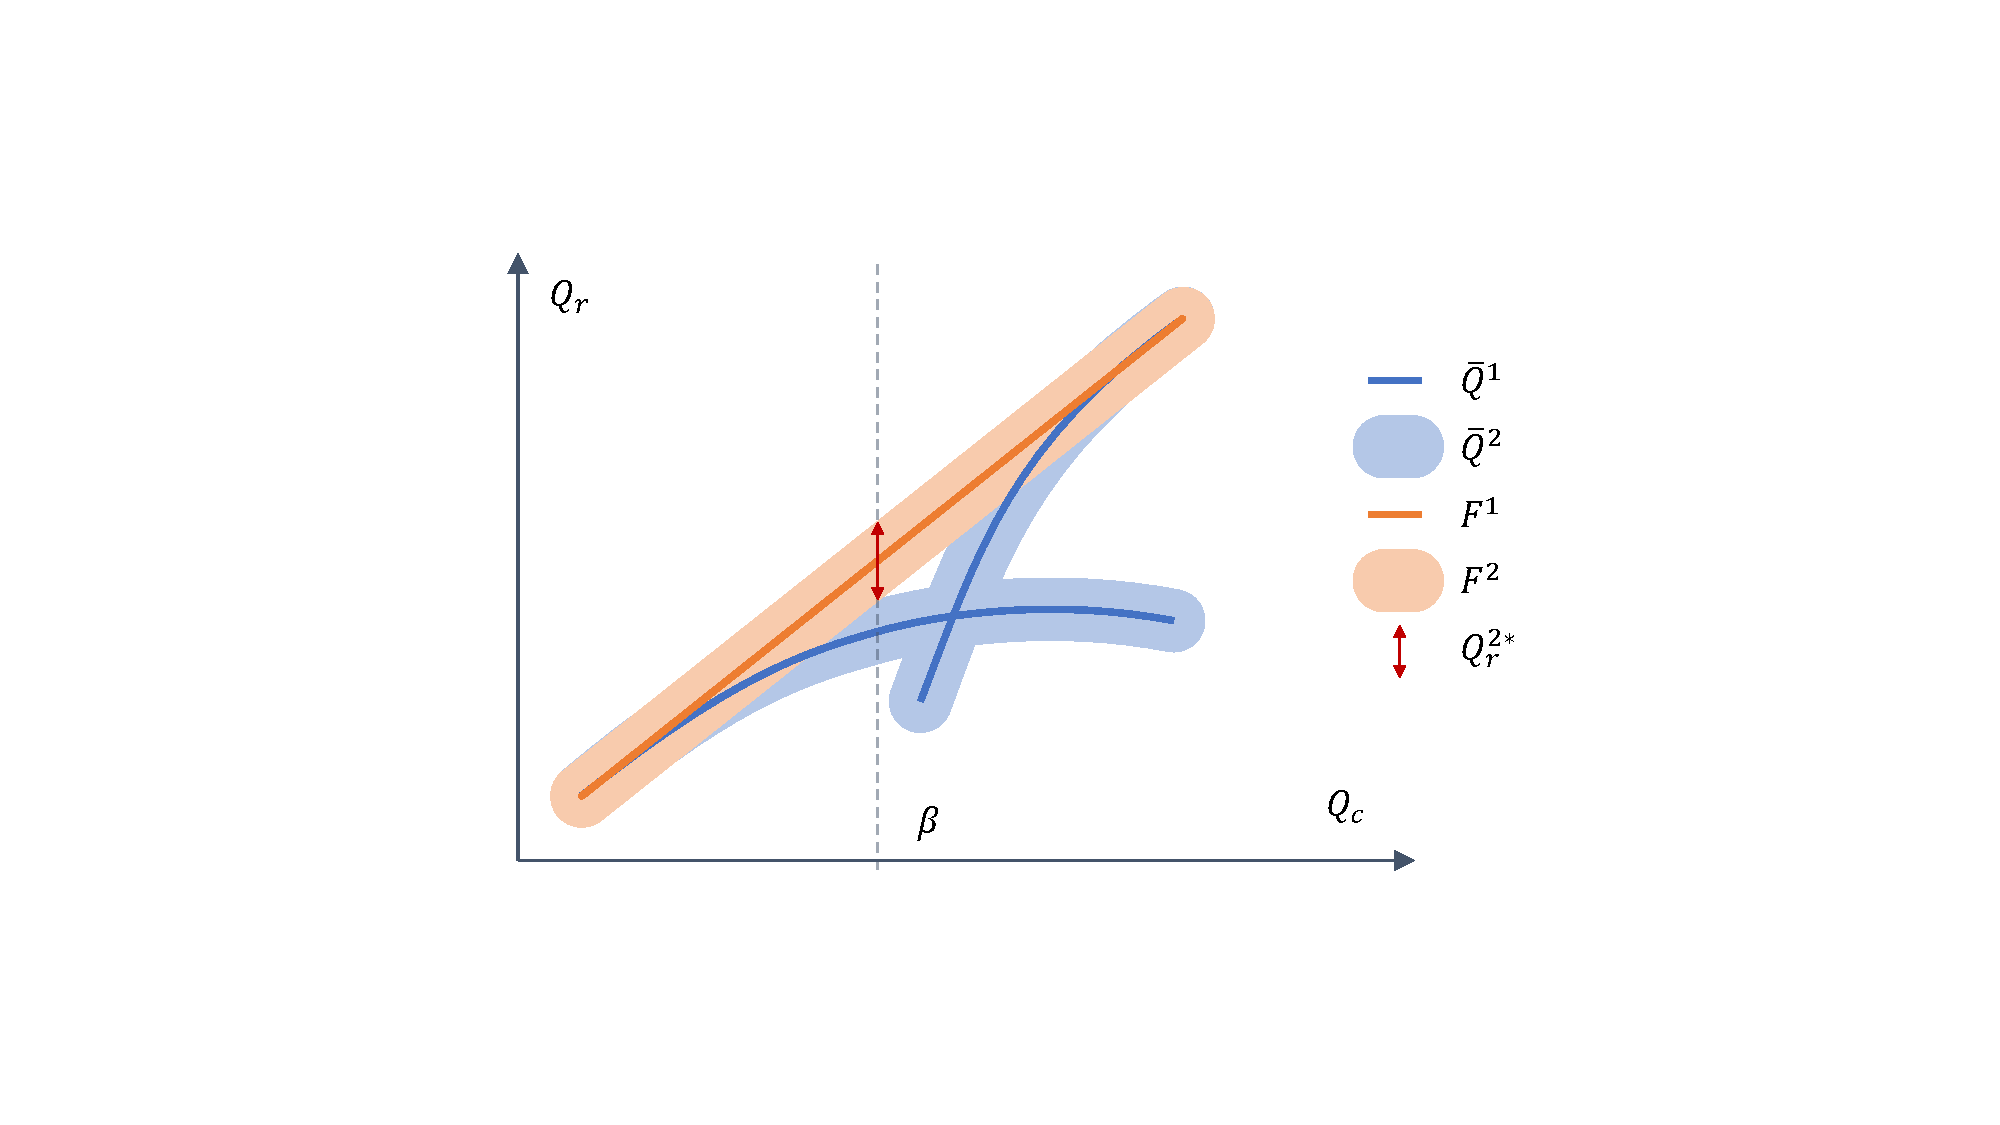
\includegraphics[trim=7cm 4cm 7cm 4cm, clip, width=0.7\textwidth]{sources/appendix/source/img/contraction_lipschitz.pdf}
        \caption{We represent the range of possible solutions $\Qr^{2,*}$ for any $\oQ^2\in\text{Ball}(\oQ^1)$, given $\oQ_1\in\cL_\lambda$}
        \label{fig:contraction_lips_hull}
    \end{figure}

    \paragraph{Step 2}

    We want to show that if $\oQ\in\cL_{\discountfactor}$, $\cF$ is the graph of an $L$-Lipschitz function:

    \begin{equation}
        \label{eq:L-lip-set}
        \forall q^1,q^2\in\cF, |q_r^2-q_r^1| \leq |q_c^2-q_c^1|.
    \end{equation}

    Let $\oQ\in\cL_{\discountfactor}$ and $\os\in\ocS$, $\cF$ the corresponding top frontier of convex hull.
    For all $q^1,q^2\in\cF, \exists \lambda,\mu\in[0,1], q^{11},q^{12},q^{21},q^{22}\in \oQ(\os,\ocA)$ such that $q^1 = (1-\lambda)q^{11} + \lambda q^{12}$ and $q^2 = (1-\mu)q^{21} + \mu q^{22}$.
    Without loss of generality, we can assume $q_c^{11}\leq q_c^{12}$ and $q_c^{21}\leq q_c^{22}$. We also consider the worst case in terms of maximum $q_r$ deviation: $q_c^{12} \leq q_c^{21}$.
    Then the maximum increment $q_r^2-q_r^{1}$ is:

    \begin{align*}
        \|q^2_r-q^{1}_r\| &\leq \|q^{12}_r-q^{1}_r\| + \|q^{21}_r-q^{12}_r\| + \|q^{2}_r-q^{21}_r\| \\
        &= (1-\lambda)\|q^{12}_r-q^{11}_r\| + \|q^{21}_r-q^{12}_r\| + \mu\|q^{22}_r-q^{21}_r\| \\
        &\leq (1-\lambda)L\|q^{12}_c-q^{11}_c\| + L\|q^{21}_c-q^{12}_c\| + \mu L\|q^{22}_c-q^{21}_c\| \\
        &= L\|q^{12}_c-q^{1}_c\| + L\|q^{21}_c-q^{12}_c\| + L\|q^{2}_c-q^{21}_c\|\\
        &= L\|q^{2}_c-q^{1}_c\|.
    \end{align*}

    This can also be seen in \Cref{fig:contraction_lips_hull}: the maximum slope of the $\cF^1$ is lower than the maximum slope between two points of $\oQ^1$.

    \paragraph{Step 3}

    Let $\cF_1$ be a L-Lipschitz set as defined in \eqref{eq:L-lip-set}, and consider a ball $\text{Ball}(\cF_1,R)$ around it as defined in \eqref{eq:ball-set}.

    We want to bound the optimal reward value $\Qr^{2*}$ under constraint $\Qc^{2*} = \budget$ (regular case in \Cref{sec:proof_pi_hull} where the constraint is saturated), for any $\cF^2\in\text{Ball}(\cF_1,R)$. This quantity is represented as a red double-ended arrow in \Cref{fig:contraction_lips_hull}.

    Because we are only interested in what happens locally at $\Qc=\budget$, we can zoom in on \Cref{fig:contraction_lips_hull} and only consider a thin $\extrasmallvalue$-section around $\budget$. In the limit $\extrasmallvalue\rightarrow 0$, this section becomes the tangent to $\cF^1$ at $\Qc^1=\budget$. It is represented in \Cref{fig:contraction_lips_hull_slope}, from which we derive a geometrical proof:

    \begin{figure}[ht]
        \centering
        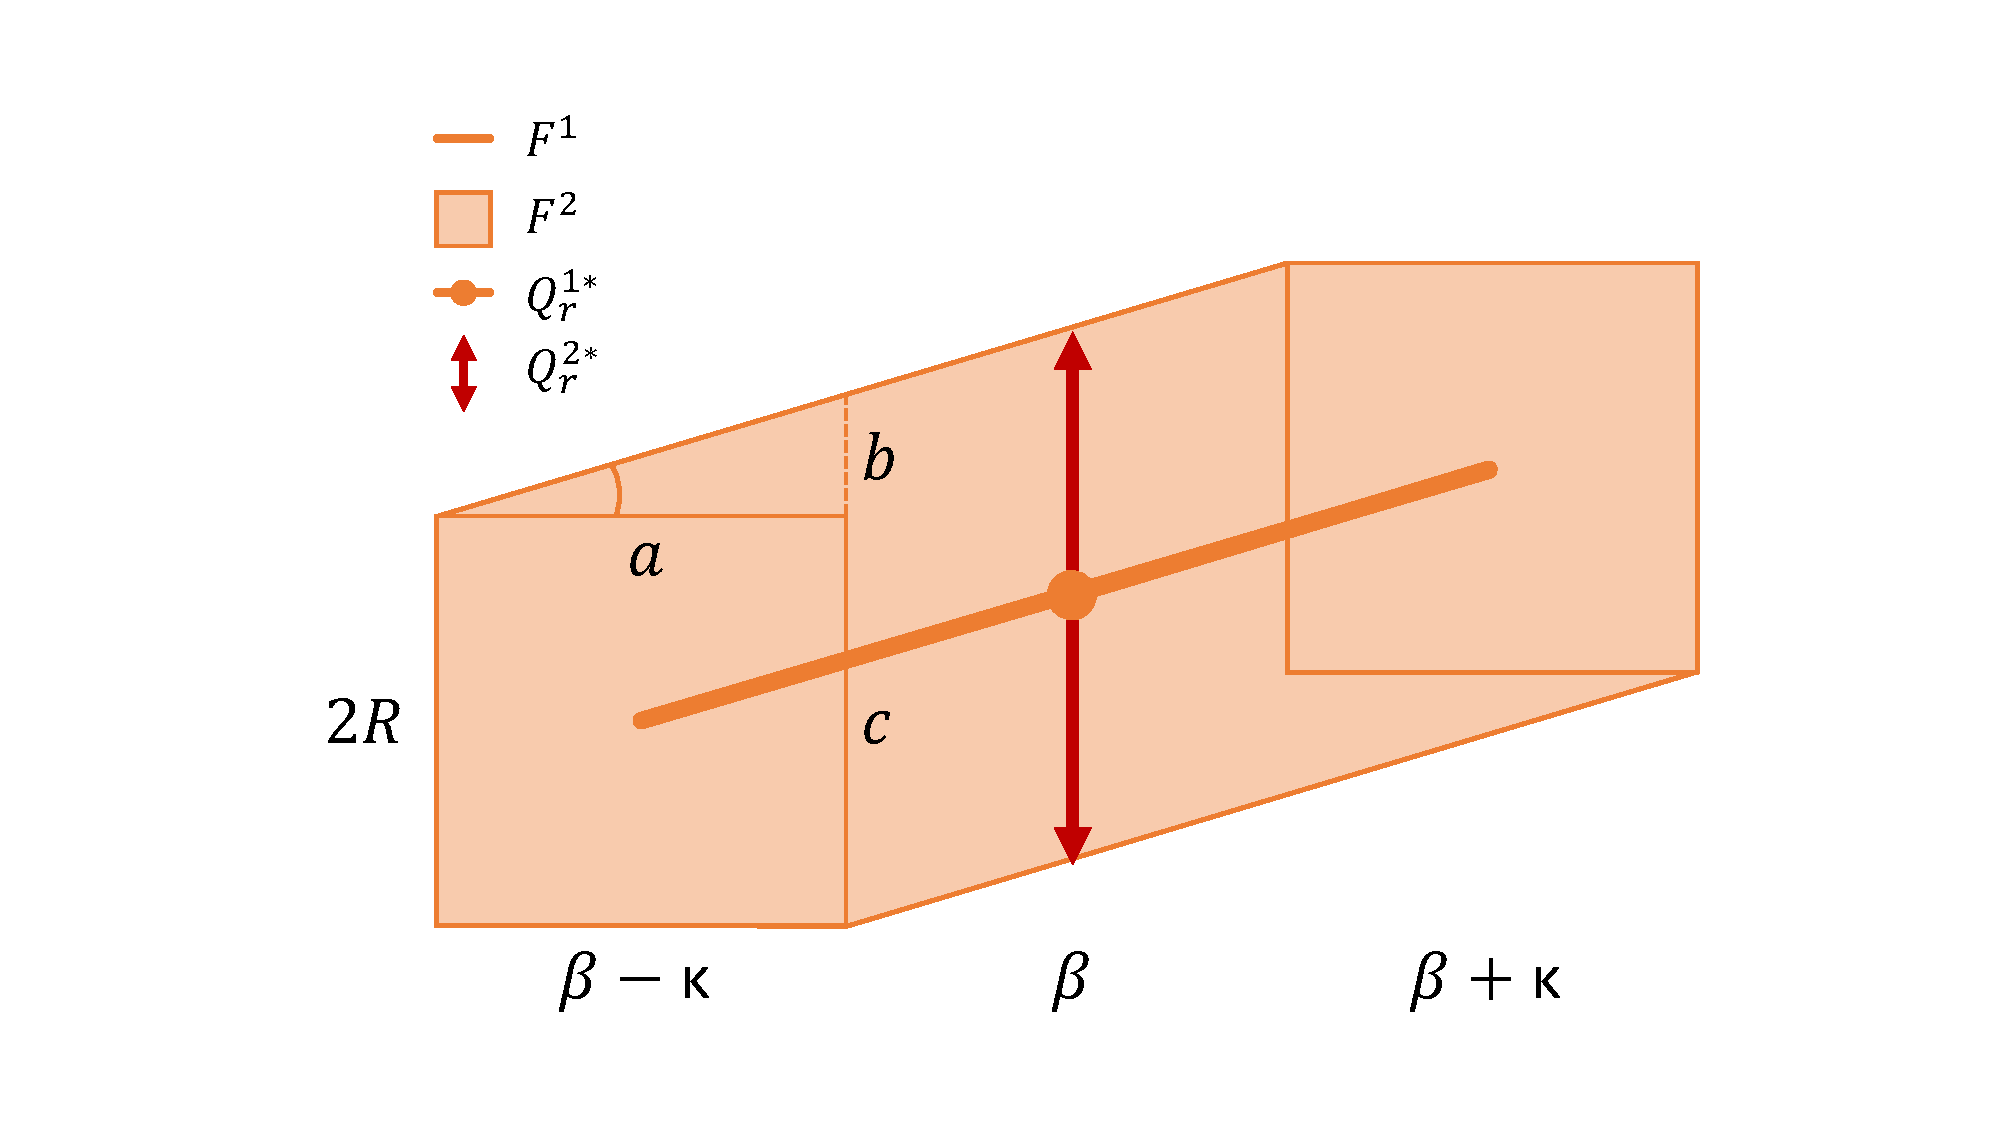
\includegraphics[trim=2cm 1cm 2cm 1cm, clip, width=0.7\textwidth]{sources/appendix/source/img/ball.pdf}
        \caption{We represent a section $[\budget-\extrasmallvalue, \budget+\extrasmallvalue]$ of $\cF^1$ and $\text{Ball}(\cF^1, R)$. We want to bound the range of $\Qr^{2*}.$}
        \label{fig:contraction_lips_hull_slope}
    \end{figure}

    \begin{align*}
        \Delta \Qr^{2*} &= b + c &\\
        & \leq La + c & \text{($\cF^1$ $L$-Lipschitz)}\\
        &= 2LR+2R = 2R(L+1).
    \end{align*}
    Hence,
    \begin{equation*}
        | \Qr^{2*} - \Qr^{1*}| \leq \frac{\Delta \Qr^{2*}}{2} = R(L+1)
    \end{equation*}

    and $\Qc^{1*} = \Qc^{2*} = \budget$.
    Consequently, $ \|\oQ^{2*} - \oQ^{1*}\|_\infty \leq (L+1)R$.

    Finally, consider the edge case in \Cref{sec:proof_pi_hull}: the constraint is not active, and the optimal value is simply $\argmax_{q\in\cF} q^r$. In particular, since we showed that $\cF^2\in \text{Ball}(\cF^1, R)$, and since $\oQ^{2*}\in \cF^2$, there exist $q^1\in \cF^1: \|\oQ^{2*}-q^1\|_\infty\leq R$ and in particular $\oQ^{1*}_r \geq q^1_r \geq \oQ^{2*}_r - R$. Reciprocally, by the same reasoning, $\Qr^{2*} \geq \Qr^{1*} - R$. Hence, we have that $| \Qr^{2*} - \Qr^{1*}| \leq R \leq R(L+1).$

    \paragraph{Wrapping it up}

    We have shown that for any $\oQ^1,\oQ^2\in\cL_{\discountfactor}$,
    and all $\os\in\ocS$, $\cF^2\in\text{Ball}(\cF^1,\|\oQ^2-\oQ^1\|_\infty)$ and $\cF^1$ is
    the graph of a $L$-Lipschitz function with $L<1/\discountfactor - 1$.
    Moreover, the solutions of $\budgetedpolicy_\text{greedy}(\oQ^1)$ and $\budgetedpolicy_\text{greedy}(\oQ^2)$ at
    $\os$ are such that $ \|\oQ^{2*} - \oQ^{1*}\|_\infty \leq (L+1)\|\oQ^2-\oQ^1\|_\infty$.

    Hence, for all $\oa$,
    \begin{align*}
        \|\abo^{*}\oQ^1(\os, \oa) - &\abo^{*}\oQ^2(\os, \oa)\|_\infty \\
        &= \discountfactor\left\|\expectedvalueover{\os'\sim\augmentedtransition(\os'|\os,\oa)}
        \expectedvalueover{\oa'\sim\budgetedpolicy_\text{greedy}(\oQ^1)}\oQ^1(\os',\oa') -
        \expectedvalueover{\oa'\sim\budgetedpolicy_\text{greedy}(\oQ^2)}\oQ^2(\os',\oa')\right\|_\infty \\
        &= \discountfactor\left\|\oQ^{2*} - \oQ^{1*}\right\|_\infty \\
        &\leq \discountfactor(L+1)\|\oQ^2-\oQ^1\|_\infty.
    \end{align*}
    Taking the sup on $\ocS\ocA$,

    \begin{equation*}
        \|\abo^{*}\oQ^1 - \abo^{*}\oQ^2\|_\infty \leq \discountfactor(L+1)\|\oQ^1-\oQ^2\|_\infty
    \end{equation*}
    with $\discountfactor(L+1) < 1$.
    As a conclusion, $\abo^{*}$ is a $\discountfactor(L+1)$-contraction on $\cL_{\discountfactor}$.
\end{proof}



\subsection{\Cref{prop:bftq_pi_hull}}

\label{sec:proof_pi_hull}

\begin{definition}
    Let $A$ be a set, and $f$ a function defined on $A$. We define:

    \begin{itemize}
        \item Convex hull of $A$: $\cC(A) = \{\sum_{i=1}^p \lambda_i a_i: a_i\in A, \lambda_i\in\Real^+, \sum_{i=1}^p \lambda_i = 1, p\in\Natural\}$
        \item Convex edges of $A$: $\cC^2(A) = \{\lambda a_1 + (1-\lambda)a_2: a_1, a_2\in A, \lambda\in[0, 1]\}$
        \item Dirac distributions of $A$: $\dirac(A) = \{\dirac(a-a_0): a_0\in A\}$
        \item Image of $A$ by $f$: $f(A) = \{f(a): a\in A\}$
    \end{itemize}
\end{definition}

\begin{proof}
    Let $\os=(s,\budget)\in\ocS$ and $\oQ\in(\Real^2)^{\ocS\ocA}$. We recall the definition of $\budgetedpolicy_\text{greedy}$:
    \begin{subequations}
        \begin{equation}
            \budgetedpolicy_\text{greedy}(\oa|\os; \oQ) \in \argmin_{\rho\in\policies_r^{\oQ}} \expectedvalueover{\oa\sim\rho}\Qc(\os, \oa) \tag{\ref{eq:pi_greedy_cost}}
        \end{equation}
        \begin{align}
            \text{where }\quad\policies_r^{\oQ} = &\argmax_{\rho\in\cM(\ocA)} \expectedvalueover{\oa\sim\rho} \Qr(\os, \oa) \tag{\ref{eq:pi_greedy_reward}}\\
            & \text{ s.t. }  \expectedvalueover{\oa\sim\rho} \Qc(\os, \oa) \leq \budget \tag{\ref{eq:pi_greedy_constraint}}
        \end{align}
    \end{subequations}

    Note that any policy in the $\argmin$ in \eqref{eq:pi_greedy_cost} is suitable to compute $\abo^{*}$.
    We first reduce the set of candidate optimal policies.
    Consider the problem described in \eqref{eq:pi_greedy_reward},\eqref{eq:pi_greedy_constraint}: it can be seen as a single-step \gls{CMDP} problem with reward $\reward=\Qr$ and cost $\constraint=\Qc$. By \parencite[Theorem 4.4][]{BEUTLER1985236}, we know that the solutions are mixtures of two deterministic policies\index{deterministic policy}. Hence, we can replace $\cM(\cA)$ by $\cC^2(\dirac(\ocA))$ in \eqref{eq:pi_greedy_reward}.

    Moreover, remark that:
    \begin{align*}
        \{\expectedvalueover{\oa\sim\rho} \oQ(\os,\oa):& \rho\in \cC^2(\dirac(\ocA))\} \\
        &= \{\expectedvalueover{\oa\sim\rho} \oQ(\os,\oa): \rho=(1-\lambda)\dirac(\oa-\oa_1)+\lambda\dirac(\oa-\oa_2), \oa_1,\oa_2\in\ocA, \lambda\in[0,1]\} \\
        &= \{(1-\lambda)\oQ(\os, \oa_1)+\lambda \oQ(\os, \oa_2), \oa_1,\oa_2\in\ocA, \lambda\in[0,1]\} \\
        &= \cC^2(\oQ(\os,\ocA))\}.
    \end{align*}

    Hence, the problem \eqref{eq:pi_greedy_reward}, \eqref{eq:pi_greedy_constraint} has become:
    \begin{equation*}
        \tilde{\policies}^{\Qr} = \argmax_{(q_r, q_c)\in\cC^2(\oQ(\os, \ocA))} q_r \quad\text{ s.t. }\quad q_c \leq \budget
    \end{equation*}
    and the solution of $\budgetedpolicy_\text{greedy}$ is $q^*=\argmin_{q\in\tilde{\policies}^{\Qr}} q_c$.

    The original problem in the space of actions $\ocA$ is now expressed in the space of values $\oQ(\os, \ocA)$ (which is why we use $=$ instead of $\in$ before $\argmin$ here).

    We further restrict the search space of $q^*$ following two observations:
    \begin{enumerate}
        \item $q^*$ belongs to the \emph{undominated} points $\cC^2(\oQ^-)$:
        \begin{align}
            \label{eq:q_minus_undominated}
            \oQ^+ &= \{(q_c, q_r): q_c > q_c^{\pm} = \min_{q^+} q_c^+\text{ s.t. }q^+\in\argmax_{q\in \oQ(\os,\ocA)} q_r\}\\
            \oQ^- &= \oQ(\os,\ocA) \setminus \oQ^+.
        \end{align}
        Denote $q^*$ = $(1-\lambda) q^1 + \lambda q^2$, with $q^1, q^2\in \oQ(\os,\ocA)$. There are three possible cases:
        \begin{enumerate}
            \item $q^1, q^2 \not\in \oQ^-$. Then $q_c^* = (1-\lambda) q^1_c + \lambda q^2_c > q_c^{\pm}$. But then $q_c^{\pm} < q_c^* \leq \budget$ so $q^{\pm}\in\tilde{\policies}^{\Qr}$ with a strictly lower $q_c$ than $q^*$, which contradicts the $\argmin$.
            \item $q^1\in \oQ^-, q^2 \not\in \oQ^-$. But then consider the mixture $q^\top = (1-\lambda) q^1 + \lambda q^\pm$. Since $q_r^{\pm} \geq q_r^{2}$ and $q_r^{\pm} < q_r^{2}$, we also have $q^\top_r \geq q_r^*$ and $q^\top_c < q_c^*$, which also contradicts the $\argmin$.
            \item $q^1,q^2\in \oQ^-$ is the only remaining possibility.
        \end{enumerate}
        \item $q^*$ belongs to the \emph{top frontier} $\cF$:
        \begin{equation}
            \label{eq:top-frontier}
            \cF_{\oQ} = \{q\in \cC^2(\oQ^-): \not\exists q'\in \cC^2(\oQ^-): q_c=q_c'\text{ and }q_r<q_r'\}.
        \end{equation}
        Trivially, otherwise q' would be a better candidate than $q^*$.
    \end{enumerate}


    Let us characterise this frontier $\cF$. It is both:
    \begin{enumerate}
        \item the \emph{graph of a non-decreasing function}: $\forall q^1, q^2\in\cF$ such that $q_c^1\leq q_c^2$ then $q_r^1\leq q_r^2$.\\
        By contradiction, if we had $q_r^1 > q_r^2$, we could define $q^\top = (1-\lambda)q^1 + \lambda q^\pm$ where $q^\pm$ is the dominant point as defined in \eqref{eq:q_minus_undominated}. By choosing $\lambda=(q^2_c-q^1_c)/(q^\pm_c-q^1_c)$ such that $q^\top_c = q_c^2$, then since $q_r^\pm \geq q_r^1 > q_r 2$ we also have $q^\top_r > q_r^2$ which contradicts $q^2\in\cF$.
        \item the \emph{graph of a concave function}: $\forall q^1, q^2, q^3\in\cF$ such that $q_c^1\leq q_c^2 \leq q_c^3$ with $\lambda$ such that $q^2_c = (1-\lambda)q^1_c + \lambda q^3_c$, then $q_r^2 \geq (1-\lambda)q_r^1 + \lambda q_r^3$.\\
        Trivially, otherwise the point $q^\top = (1-\lambda)q^1 + \lambda q^3$ would verify $q^\top_c=q^2_c$ and $q^\top_r > q^2_r$, which would contradict $q^2 \in\cF$.
    \end{enumerate}

    We denote $\cF_{\oQ} = \cF \cap \oQ$. Clearly, $q^*\in\cC^2(\cF_{\oQ})$: let $q^1, q^2\in \oQ^-$ such that $q^* = (1-\lambda)q^1 + \lambda q^2$. First, $q^1, q^2\in \oQ^-\subset\cC^2(\oQ^-)$. Then, by contradiction, if there existed $q^{1'}$ or $q^{2'}$ with equal $q_c$ and strictly higher $q_r$, again we could build an admissible mixture $q^{\top}=(1-\lambda)q^{1'}  + \lambda q^{2'}$ strictly better than $q^*$.

    $q^*$ can be written as $q^* = (1-\lambda)q^1 + \lambda q^2$ with $q^1, q^2\in\cF_{\oQ}$ and, without loss of generality, $q^1_c \leq q^2_c$.

    \paragraph{Regular case}

    There exists $q^0\in\cF_{\oQ}$ such that $q^0_c \geq \budget$. Then $q^1$ and $q^2$ must flank the \idx{budget}: $q_c^1 \leq \budget \leq q_c^2$. Indeed, by contradiction, if $q_c^2 \geq q_c^1 > \budget$ then $q_c^* > \budget$ which contradicts $\policies_r^{\oQ}$. Conversely, if $q_c^1 \leq q_c^2 < \budget$ then $q^* < \budget \leq q^0_c$, which would make $q^*$ a worse candidate than $q^\top=(1-\lambda)q^* + \lambda q^0$ when $\lambda$ is chosen such that $q_c^\top=\budget$, and contradict $\policies_r^{\oQ}$ again.

    Because $\cF$ is the graph of a non-decreasing function, $\lambda$ should be as high as possible, as long as the \idx{budget} $q^*\leq\budget$ is respected. We reach the highest $q_r^*$ when $q^*_c=\budget$, that is: $\lambda=(\budget-q_c^1)/(q_c^2-q_c^1)$.

    It remains to show that $q^1$ and $q^2$ are two successive points in $\cF_{\oQ}$: $\not\exists q\in\cF_{\oQ}\setminus\{q^1, q^2\}: q^1_c \leq q_c \leq q^2_c$. Otherwise, as $\cF$ is the graph of a concave function, we would have $q_r \geq (1-\mu)q_r^1 + \mu q_r^2$. $q_r$ cannot be strictly greater than $(1-\mu)q_r^1 + \mu q_r^2$ which would contradict $q^*$, but it can still be equal, which means the tree points $q, q^1, q^2$ are aligned. In fact, every points aligned with $q^1$ and $q^2$ can also be used to construct mixtures resulting in $q^*$, but among these solutions we can still choose $q^1$ and $q^2$ as the two points in $\cF_{\oQ}$ closest to $q^*$.

    \paragraph{Edge case}

    $\forall q\in\cF_{\oQ}, q_c < \budget$. Then  $q^* =  \argmax_{q\in\cF} q_r = q^\pm =  \argmax_{q\in \oQ^-} q_r$.
\end{proof}

\section{Parameters}
\label{sec:params:appendix}

All algorithm parameters are displayed in \Cref{tab:param-algo-corridors},\Cref{tab:param-algo-slot-filling} and \Cref{tab:param-algo-highway-env}.


\paragraph{State-Space}

The states $s$ (from $\os=(s,\budget)$) of the \idx{agent} are described in the following:

\begin{itemize}
    \item \texttt{Corridors}: $s = (x,y)$ where $x$ and $y$ are the 2D coordinates of the \idx{agent}.
    \item \texttt{\idx{slot-filling}}: $s = (\srs,\text{min},a_u,a_s,t)$ where $\srs$ is a vector of the \gls{SRS} for each slot, $\text{min}$ is a one hot vector describing the minimum of the $\srs$ vector, $a_u$ is a one hot vector of the last \idx{user} \idx{dialogue act} and $a_s$ is the one hot vector of the last system \idx{dialogue act}. Finally $t\in[0,1]$ is the fraction of the current \idx{turn} with the maximum number of \idx{turn}s authorised.
    \item \texttt{Highway-Env}: the positions $(x, y)$ and velocities $(\dot{x}, \dot{y})$ of every vehicle on the road.
\end{itemize}


\paragraph{A note on the parameters search}

We performed a shallow grid-search for the classic \gls{NN} parameters. Most of the parameters do not have a strong influence on the results, however in the \texttt{\idx{slot-filling}} \idx{environment}, the choice of the regulation weight is decisive.

\begin{table}[tp]
    \centering
    \begin{tabularx}{1.0\textwidth}{lll}
        \toprule
        Parameters & \gls{BFTQ}(\idx{risk-sensitive}) & \gls{BFTQ}(\idx{risk-neutral})\tabularnewline
        \midrule
        architecture & 256x128x64 & 256x128x64\tabularnewline
        regularisation & 0.001 & 0.001\tabularnewline
        activation & relu & relu\tabularnewline
        size beta encoder & 3 & 3\tabularnewline
        initialisation & xavier & xavier\tabularnewline
        loss function & L2 & L2\tabularnewline
        optimizer & adam & adam\tabularnewline
        learning rate & 0.001 & 0.001\tabularnewline
        epoch (\gls{NN}) & 1000 & 5000\tabularnewline
        normalize reward & true & true\tabularnewline
        epoch (\gls{FTQ}) & 12 & 12\tabularnewline
        $\tilde{\budgetspace}$ & 0:0.01:1 & -\tabularnewline
        $\discountfactor$ & 1 & 1\tabularnewline
        $\T=|\cD|$ & 5000 & 5000\tabularnewline
        $N_\text{minibatch}$ & 10 & 10\tabularnewline
        $N_\text{seeds}$ & 4 & 4\tabularnewline
        $N_\text{test}$ & 1000 & 1000\tabularnewline
        decay epsilon scheduling & 0.001 & 0.001\tabularnewline
        \bottomrule

    \end{tabularx}
    \caption{Algorithms parameters for \texttt{Corridors}}
    \label{tab:param-algo-corridors}
\end{table}

\begin{table}[tp]
    \centering
    \begin{tabularx}{1.0\textwidth}{lll}
        \toprule
        Parameters & \gls{BFTQ} & \gls{FTQ}\tabularnewline
        \midrule
        architecture & 256x128x64 & 128x64x32\tabularnewline
        regularisation & 0.0005 & 0.0005\tabularnewline
        activation & relu & relu\tabularnewline
        size beta encoder & 50 & -\tabularnewline
        initialisation & xavier & xavier\tabularnewline
        loss function & L2 & L2\tabularnewline
        optimizer & adam & adam\tabularnewline
        learning rate & 0.001 & 0.001\tabularnewline
        epoch (\gls{NN}) & 5000 & 5000\tabularnewline
        normalize reward & true & true\tabularnewline
        epoch (\gls{FTQ}) & 11 & 11\tabularnewline
        $\tilde{\budgetspace}$ & 0:0.01:1 & -\tabularnewline
        $\discountfactor$ & 1 & 1\tabularnewline
        $\T=|\cD|$ & 5000 & 5000\tabularnewline
        $N_\text{minibatch}$ & 10 & 10\tabularnewline
        $N_\text{seeds}$ & 6 & 6\tabularnewline
        $N_\text{test}$ & 1000 & 1000\tabularnewline
        decay epsilon scheduling & 0.001 & 0.001\tabularnewline
        \bottomrule
    \end{tabularx}
    \caption{Algorithms parameters for \texttt{slot-filling}}
    \label{tab:param-algo-slot-filling}
\end{table}
\begin{table}[tp]
    \centering
    \begin{tabularx}{1.0\textwidth}{lll}
        \toprule
        Parameters & \gls{BFTQ} & \gls{FTQ}\tabularnewline
        \midrule
        architecture & 256x128x64 & 128x64x32\tabularnewline
        regularisation & 0.0005 & 0\tabularnewline
        activation & relu & relu\tabularnewline
        size beta encoder & 50 & -\tabularnewline
        initialisation & xavier & xavier\tabularnewline
        loss function & L2 & L2\tabularnewline
        optimizer & adam & adam\tabularnewline
        learning rate & 0.001 & 0.01\tabularnewline
        epoch (\gls{NN}) & 5000 & 400\tabularnewline
        normalize reward & true & true\tabularnewline
        epoch (\gls{FTQ}) & 15 & 15\tabularnewline
        $\tilde{\budgetspace}$ & 0:0.01:1 & -\tabularnewline
        $\discountfactor$ & 0.9 & 0.9\tabularnewline
        $\T=|\cD|$ & 10000 & 10000\tabularnewline
        $N_\text{minibatch}$ & 10 & 10\tabularnewline
        $N_\text{seeds}$ & 10 & 10\tabularnewline
        $N_\text{test}$ & 150 & 150\tabularnewline
        decay epsilon scheduling & 0.0003 & 0.0003\tabularnewline
        \bottomrule
    \end{tabularx}
    \caption{Algorithms parameters for \texttt{Highway-Env}}
    \label{tab:param-algo-highway-env}
\end{table}

\section{Repoducibility}

\subsection{Instructions for reproducibility}
\label{subsubsec:instruction-reproducibility}
To reproduce the result displayed in \Cref{sec:experiements}, first install the following conventional libraries for python3: pycairo, numpy, scipy and pytorch. Then, on a Linux Operating System, execute the following commands:\\
\\
\begin{minipage}{\linewidth}
    \begin{lstlisting}[language=bash,label={fig:instructions},title={Instructions to reproduce experiments},breaklines,captionpos=b]
        # Install highway-env
        pip3 install --user git+https://github.com/eleurent/rl-agents
        # Change python path to the path of this repository
        export PYTHONPATH="code/scaling-up-brl"
        # pull code
        git clone https://github.com/scaling-up-brl/scaling-up-brl.github.io.git
        # Navigate to budgeted-rl folder
        cd scaling-up-brl.github.io/code/scaling-up-brl/budgeted-rl/
        # Run main script using any config file
        # Choose the range of seeds you want to test on
        python3 main/egreedy/main-egreedy.py config/slot-filling.json 0 6
        python3 main/egreedy/main-egreedy.py config/corridors.json 0 4
        python3 main/egreedy/main-egreedy.py config/highway-easy.json 0 10
    \end{lstlisting}
\end{minipage}

The \gls{GPU} used for experiments is an NVIDIA \texttt{GeForce GTX 1080 Ti} and the \gls{CPU} is an Intel \texttt{Xeon E7}.


\subsection{The Machine Learning reproducibility checklist}
\label{sec:ml-checklist}
For all models\index{model} and algorithms presented, indicate if you include:

\begin{itemize}
    \item  A clear description of the mathematical setting, algorithm, and/or \idx{model}:

    \begin{itemize}
        \item \textbf{yes}, see \Cref{sec:intro}, \Cref{sec:bdp}, \Cref{sec:brl},
        and \Cref{sec:scalable-bftq}.
    \end{itemize}
    \item An analysis of the complexity (time, space, sample size) of any algorithm:
    \begin{itemize}
        \item \textbf{yes}, see \Cref{subsec:parallel-computing}.
    \end{itemize}
    \item A link to a downloadable source code, with specification of all dependencies, including external libraries:
    \begin{itemize}
        \item \textbf{yes}, see \Cref{subsubsec:instruction-reproducibility} and the folder \texttt{code} in the supplementary material zip file.
    \end{itemize}
\end{itemize}

For any theoretical claim, indicate if you include:

\begin{itemize}
    \item  A statement of the result:
    \begin{itemize}
        \item  \textbf{yes}, see \Cref{sec:bdp} and \Cref{sec:brl}.
    \end{itemize}
    \item A clear explanation of any assumptions:
    \begin{itemize}
        \item  we make one assumption in \Cref{sec:bdp}. We assume the program is feasible for any state. If not, no algorithm would be able to solve it anyway.
    \end{itemize}
    \item A complete proof of the claim:
    \begin{itemize}
        \item  \textbf{yes}, see \Cref{sec:proofs}.
    \end{itemize}
\end{itemize}

For all figures and tables that present empirical results, indicate if you include:

\begin{itemize}
    \item A complete description of the data collection process, including sample size:

    \begin{itemize}
        \item\textbf{yes}, see \Cref{sec:experiements} and \Cref{sec:params:appendix}.
    \end{itemize}
    \item A link to a downloadable version of the dataset or simulation \idx{environment}:

    \begin{itemize}
        \item  \textbf{yes}, all \idx{environment}s are fetch from a public repository, see \Cref{subsubsec:instruction-reproducibility} for details.
    \end{itemize}
    \item An explanation of any data that were excluded, description of any pre-processing step:
    \begin{itemize}
        \item it is \textbf{not applicable} as data comes from simulated \idx{environment}s, so pre-processing steps are not needed.
    \end{itemize}

    \item An explanation of how samples were allocated for training / validation / testing:
    \begin{itemize}
        \item it is \textbf{not applicable}. The complete dataset is used for training. There is no need for validation set. Testing is performed in the true \idx{environment} as in classical \idx{Online} learning approaches.
    \end{itemize}

    \item The range of hyper-parameters considered, method to select the best hyper-parameter configuration, and specification of all hyper-parameters used to generate results:

    \begin{itemize}
        \item \textbf{yes}, see \Cref{sec:params:appendix}.
    \end{itemize}

    \item The exact number of evaluation runs:

    \begin{itemize}
        \item \textbf{yes}, see $N_{seeds}$ in the tables from \Cref{sec:params:appendix}.
    \end{itemize}

    \item A description of how experiments were run:
    \item
    \begin{itemize}
        \item \textbf{yes}, see the two first paragraphs of \Cref{par:ex-explo}.
    \end{itemize}

    \item A clear definition of the specific measure or statistics used to report results:
    \begin{itemize}
        \item  \textbf{yes}, see \Cref{subsec:results}.
    \end{itemize}

    \item Clearly defined error bars:

    \begin{itemize}
        \item  \textbf{yes}, we plot 95\% confidence intervals in all figures, see \Cref{subsec:results}.
    \end{itemize}

    \item A description of results with central tendency (e.g. mean)  variation (e.g. stddev):

    \begin{itemize}
        \item  \textbf{yes}, we even observe less variability with our novel approach, see \Cref{subsec:results}.
    \end{itemize}
    \item A description of the computing infrastructure used:
    \begin{itemize}
        \item The \gls{GPU} used for experiments is an NVIDIA \texttt{GeForce GTX 1080 Ti} and the \gls{CPU} is an Intel \texttt{Xeon E7}.
    \end{itemize}
\end{itemize}